%!TEX root = informe.tex
\chapter{Análisis de Ciclo de Vida: instalación, uso y mantenimiento}
%(Fuente: Manual Técnico para la correcta colocación de los Euroadoquines (MTCE 04))
\section{Introducción}
La correcta colocación y mantenimiento del pavimento con adoquines es igual de importante que la calidad en los materiales y los procesos de fabricación \cite{euroadoquinc} para que el funcionamiento del pavimento sea el adecuado.

Hay múltiples manuales y guías técnicas que explican los criterios prácticos y recomendaciones para una correcta colocación de los adoquines.

La planificación del trabajo empieza estudiando el tipo de vía y uso principal al que estará destinado el pavimento. Una vez decidido es necesario preparar la explanada y las diferentes capas componentes en función de ese uso. A continuación se coloca la capa de adoquines, se sella con arena y se realiza un vibrado del pavimento. Por último se realiza una limpieza final.

\section{Capas componentes}

\begin{itemize}
\item Explanada: Terreno natural adecuadamente compactado hasta alcanzar una capacidad portante mínima.
\item Subbase: Conjunto de capas naturales, de material granular seleccionado, estabilizado y compactado, situadas directamente sobre la explanada.
\item Base: Principal elemento portante de la estructura, situada sobre la subbase. Puede ser realizada con material granular, zahorra artificial, con un mayor grado de compactación que el alcanzado en la subbase (Base Flexible), o estar realizada con hormigón magro (Base Rígida).
\item Lecho de árido: Base de apoyo de los adoquines, destinada a absorber sus diferencias de espesor debidas a la tolerancia de fabricación, de manera que estos una vez compactados formen una superficie homogénea.
\item Adoquines: Elementos prefabricados de hormigón, cuya cara exterior, una vez colocados, forman la capa de rodadura de la superficie a pavimentar.
\item Relleno final: Una vez encastrados en el lecho de árido, sus juntas precisan un relleno final para transferir a los elementos contiguos las cargas a las que sean sometidos por acción del tráfico.
\end{itemize}

\section{Determinación de la sección tipo}\label{sec:secciontipo}

Se consideran los siguientes casos:

\begin{enumerate}
\item Viales y zonas de aparcamiento\footnote{No suelen existir zonas peatonales puras (paso eventual de vehículos de mantenimiento, limpieza y servicios).}.
\item Zonas industriales.
\end{enumerate}


Para cada caso, viales o zonas industriales, la sección puede obtenerse de forma abreviada en función de dos variables:
\begin{itemize}
\item Tipo de explanadas.
\item Categoría de tráfico.
\end{itemize}

\subsection{Tipo de explanada}

Se utiliza un sistema de clasificación de su capacidad portante mediante el índice CBR (California Bearing Ratio), indicando el tanto por ciento de la presión ejercida por un pistón sobre el suelo para alcanzar una determinada penetración baremado según un juego de muestras normalizados (ver tabla \ref{indicecbr}.

\begin{table}[!htb]
\centering
\begin{tabular}{cc}
\toprule
Calidad de la explanada & Índice CBR\\
\midrule
E1 & 5 $\leq$ CBR = 10\\
E2 & 10 $\leq$ CBR = 20\\
E3 & 20 $\leq$ CBR\\
\bottomrule
\end{tabular}
\caption{Índice CBR.}
\label{indicecbr}
\end{table}


\subsection{Categoría de tráfico}

\begin{table}[!htb]
\centering
\begin{tabular}{cc}
\toprule
Tipo & Categoría de tráfico\\
\midrule
Viales y zonas de aparcamiento & C0 \ldots C4\\
Zonas industriales & A \ldots D\\
\bottomrule
\end{tabular}
\caption{Categoría de tráfico.}
\label{categoriadetrafico}
\end{table}

\subsubsection{Categorías de tráfico en viales y zonas de aparcamiento}

Si en un área limitada existen diversos usos, a efectos de unificación se debería emplear para toda la zona la carga de cálculo más exigente.

\begin{table}[!htb]
\centering
\begin{tabular}{p{7cm}c}
\toprule
Uso previsto & Categoría de tráfico\\
\midrule
Arterias principales con gran afluencia de tráfico, paradas de bus, estaciones de servicio, etc. (50 a 149 v.p.d.) & C0\\
Arterias principales (25 a 49 v.p.d.) & C1\\
Calles comerciales con gran actividad (16 a 24 v.p.d.) & C2\\
Calles comerciales cone escasa actividad (15 v.p.d.) & C3\\
Áreas peatonales, calles residenciales & C4\\
\bottomrule
\end{tabular}
\caption{Categoría de tráfico en viales y zonas de aparcamiento.}
\label{categoriadetraficoenviales}
\end{table}


\subsubsection{Categorías de tráfico en zonas industriales}

\begin{table}[!htb]
\centering
\begin{tabular}{cccc}
\toprule
\multicolumn{2}{c}{Área} & Uso & Intensidad de uso\\
\midrule
\multirow{7}{*}{Comercial} & De operación & — & Alta\\
& \multirow{2}{*}{Almacenamiento} & Mercancia convencional & Media\\
& & Mercancía pesada & Alta\\
& Manipulación & — & Alta\\
& \multirow{3}{*}{Estacionamiento} & Vehículos pesados y ligeros & Media\\
& & Vehículos pesados exclusivamente & Alta\\
& & Semirremolques & Alta\\
\midrule
\multirow{3}{*}{Militar} & De operación & — & Alta\\
& \multirow{2}{*}{Almacenamiento} & Mercancia convencional & Media\\
& & Mercancía pesada y semirremolques & Alta\\
\midrule
\multirow{3}{*}{Pesquera} & Almacenamiento & — & Media\\
& Manipulación & — & Alta\\
& Clasificación y venta & — & Media\\
\midrule
\multirow{3}{*}{Industrial} & De operación & — & Alta\\
& \multirow{2}{*}{Almacenamiento} & Mercancia convencional & Media\\
& & Mercancía pesada & Alta\\
\bottomrule
\end{tabular}
\caption{Intensidades de uso en zonas industriales.}
\label{categoriadetraficoenzonasindustrialesintensidades}
\end{table}


\begin{table}[!htb]
\centering
\begin{tabular}{cccc}
\toprule
Intensidad de uso & \multicolumn{3}{c}{Carga de cálculo}\\
\cmidrule{2-4}
& Alta & Media & Baja\\
\midrule
Elevada & A & B & C\\
Media & A & B & D\\
Reducida & B & C & D\\
\bottomrule
\end{tabular}
\caption{Categoría de tráfico en zonas industriales.}
\label{categoriadetraficoenzonasindustriales}
\end{table}

\section{Secciones tipo}

Las secciones tipo según la base y el uso previsto del área vistas en la sección \ref{sec:secciontipo} pueden resumirse en cinco tipos para cada tipo de base, granular (figura \ref{fig:seccionestipogranular}) u hormigón magro (figura \ref{fig:seccionestipohormigon}).

\begin{figure}[!htb]
\centering
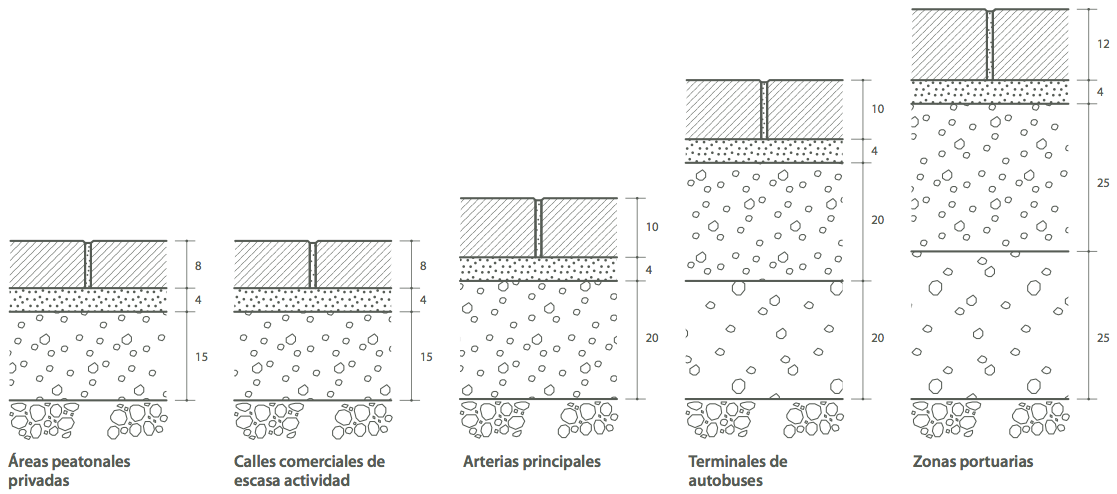
\includegraphics[width=15cm]{seccionestipo_1.png}
\caption[Secciones tipo para base granular.]{Secciones tipo para base granular. Unidades en cm. Fuente: \cite{fenollar}.}
\label{fig:seccionestipogranular}
\end{figure}

\begin{figure}[!htb]
\centering
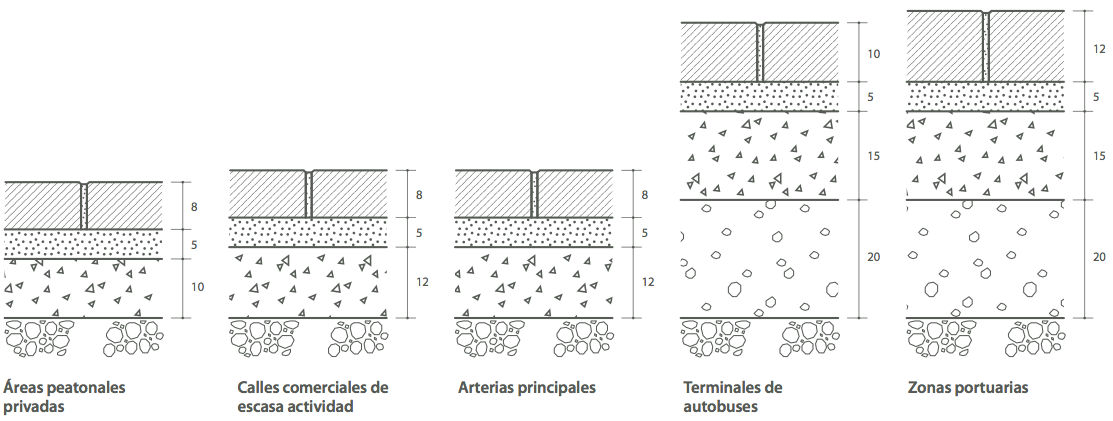
\includegraphics[width=15cm]{seccionestipo_2.png}
\caption[Secciones tipo para base de hormigón.]{Secciones tipo para base de hormigón. Unidades en cm. Fuente: \cite{fenollar}.}
\label{fig:seccionestipohormigon}
\end{figure}

\section{Modelado de los procesos}

Debido a que hay múltiples tipos de vía y uso destinado, se ha optado para el presente proyecto modelar la instalación más común, \textit{arterias principales}, que pertenece a la \textit{categoría de tráfico C1} y una \textit{calidad de explanada E2} con una base granular. Con esta clasificación, siguiendo las recomendaciones de \cite{euroadoquinc} el corte del terreno 1 \si{m^2} de superficie de terreno, que es la Unidad Funcional, será el reflejado en la tabla \ref{cortedelterreno}.

\begin{table}[!htb]
\centering
\begin{tabular}{lrrr}
\toprule
\multicolumn{4}{c}{Capas componentes para arterías principales C1-E2 con base granular}\\
\midrule
Capa componente & Grosor (\si{cm}) & Densidad (\si{kg/m^3}) & Volumen (\si{m^3})\\
\midrule
Adoquín \& Sellado & 10 & 2650 & 0.1\\
Lecho de árido & 4 & 1650 & 0.04\\
Base granular & 20 & 1500 & 0.2\\
Subbase & — & — & —\\
Explanada & \multicolumn{3}{c}{Aplanar y compactar}\\
\midrule
Total & 34 & — & 0.34\\
\bottomrule
\end{tabular}
\caption{Capas componentes para arterías principales C1-E2 con base granular.}
\label{cortedelterreno}
\end{table}

\subsection{Árido grueso para base granular (zahorra)}
1500kg/m3
Gravel, crushed, at mine/CH U 300
Transport, lorry 16-32t, EURO4/RER U 300 50

La arena para sellado debe ser una arena sin exceso de finos, ya que si existen demasiados finos, se producirá un vaciado de las juntas con el uso y limpieza del pavimento o bien se filtrarás hacia el lecho.

Además debe ser libre de sales solubles y otros contaminantes, ya que pueden provocar la aparición de eflorescencias —igual que en el caso del lecho de árido—.

No se debe usar mortero para el sellado de las juntas, ya que no se podrán retirar para hacer tareas de mantenimiento —principal ventaja de los adoquines de hormigón—, además de perder flexibilidad del conjunto.

La arena de sílice —\textit{Silica sand}, en inglés— es un material adecuado para esta tarea \cite{website:cement}. SimaPro pide como parámetro la masa de arena que se empleará para el rellenado. Si se tiene en cuenta que el adoquín mide 10 \si{cm} de altura, 1 \si{cm} quedará enterrado en el lecho, y se añadirá 1 \si{cm} por encima para el vibrado; por otro lado, la junta medirá 5 \si{mm}, se puede obtener el volumen y a partir de él la masa:

\begin{gather}
1 m^2 = 50 \text{ adoquines} = 10 \times 5\\
Adoquin = 20 \times 10 \times 6 cm\\
\delta_{junta} = 0.5cm\\
Largo = 10 \times 10 + 9 \times 0.5 = 104.5 cm\\
Ancho = 5 \times 20 + 4 \times 0.5 = 102 cm\\
\text{Superficie de arena} = 104.5 \times 0.5 + 102 \times 0.5 = 103.25 cm^2\\
\text{Volumen de arena} = 103.25 \times 10 = 1032.5 cm^3\\
\rho_{arena}=2.6 g/cm^3\\
\text{Masa de arena} = 1032.5 \times 2.65 = 2.74 kg
\end{gather}

Por otro lado, si se supone una distancia de entrega de 50 km hasta el destino de la instalación en un camión de transporte, se tiene:

\begin{equation}
2.74 kg \times 50 km = 137 kg \times km
\end{equation}

\begin{table}[!htb]
\centering
\begin{tabular}{p{8cm}rc}
\toprule
\multicolumn{3}{c}{Arena para sellado}\\
\midrule
Materiales/Ensamblajes & Cantidad & Unidad\\
\midrule
Silica sand, at plant/DE U & 2.74 & \si{kg}\\
\midrule
Procesos & Cantidad & Unidad\\
\midrule
Transport, lorry 16-32t, EURO4/RER U & 137 & \si{kg\times km}\\
\bottomrule
\end{tabular}
\caption{Modelado de la arena para sellado.}
\label{modeladoarenasellado}
\end{table}

\subsection{Árido semi-fino para lecho de arena}

Sand, at mine/CH U 66
1650 kgm3
Transport 66*50

\subsection{Arena para sellado}

La arena para sellado debe ser una arena sin exceso de finos, ya que si existen demasiados finos, se producirá un vaciado de las juntas con el uso y limpieza del pavimento o bien se filtrarás hacia el lecho.

Además debe ser libre de sales solubles y otros contaminantes, ya que pueden provocar la aparición de eflorescencias —igual que en el caso del lecho de árido—.

No se debe usar mortero para el sellado de las juntas, ya que no se podrán retirar para hacer tareas de mantenimiento —principal ventaja de los adoquines de hormigón—, además de perder flexibilidad del conjunto.

La arena de sílice —\textit{Silica sand}, en inglés— es un material adecuado para esta tarea \cite{website:cement}. SimaPro pide como parámetro la masa de arena que se empleará para el rellenado. Si se tiene en cuenta que el adoquín mide 10 \si{cm} de altura, 1 \si{cm} quedará enterrado en el lecho, y se añadirá 1 \si{cm} por encima para el vibrado; por otro lado, la junta medirá 5 \si{mm}, se puede obtener el volumen y a partir de él la masa:

\begin{gather}
1 m^2 = 50 \text{ adoquines} = 10 \times 5\\
Adoquin = 20 \times 10 \times 6 cm\\
\delta_{junta} = 0.5cm\\
Largo = 10 \times 10 + 9 \times 0.5 = 104.5 cm\\
Ancho = 5 \times 20 + 4 \times 0.5 = 102 cm\\
\text{Superficie de arena} = 104.5 \times 0.5 + 102 \times 0.5 = 103.25 cm^2\\
\text{Volumen de arena} = 103.25 \times 10 = 1032.5 cm^3\\
\rho_{arena}=2.6 g/cm^3\\
\text{Masa de arena} = 1032.5 \times 2.65 = 2.74 kg
\end{gather}

Por otro lado, si se supone una distancia de entrega de 50 km hasta el destino de la instalación en un camión de transporte, se tiene:

\begin{equation}
2.74 kg \times 50 km = 137 kg \times km
\end{equation}

\begin{table}[!htb]
\centering
\begin{tabular}{p{8cm}rc}
\toprule
\multicolumn{3}{c}{Arena para sellado}\\
\midrule
Materiales/Ensamblajes & Cantidad & Unidad\\
\midrule
Silica sand, at plant/DE U & 2.74 & \si{kg}\\
\midrule
Procesos & Cantidad & Unidad\\
\midrule
Transport, lorry 16-32t, EURO4/RER U & 137 & \si{kg\times km}\\
\bottomrule
\end{tabular}
\caption{Modelado de la arena para sellado.}
\label{modeladoarenasellado}
\end{table}

\subsection{Excavación del terreno}

A la hora de realizar un pavimento de adoquines, se debe realizar en primer lugar la excavación del terreno. Dado que el grosor total de las capas componentes es de 34 \si{cm} y se dispone de un área de 1 \si{m^2}, el volumen a introducir para el modelo será 0.34 \si{m^3}, utilizando como entrada de SimaPro de excavación con herramienta hidráulica, \textit{Excavation, hydraulic digger}.

\begin{table}[!htb]
\centering
\begin{tabular}{p{8cm}rc}
\toprule
\multicolumn{3}{c}{Excavación del terreno}\\
\midrule
Materiales/combustibles & Cantidad & Unidad\\
\midrule
Excavation, hydraulic digger/RER U & 0.34 & \si{m^3}\\
\bottomrule
\end{tabular}
\caption{Modelado de la excavación del terreno.}
\label{modeladoexcavacion}
\end{table}

\subsection{Compactación de la explanada}

Una vez excavado el terreno es necesario compactar lo que será la explanada. La bibliografía consultada no ha ofrecido ninguna solución óptima a este tipo de proceso, por lo que se ha optado por asemejar el tipo de trabajo de un tractor usando un rodillo para cultivar la tierra —\textit{Tillage, rolling}, en inglés— con el rodillo utilizado por una apisonadora o compactadora —\textit{road roller}, en inglés—. En este caso, la compactación se realiza en unidades de área, por lo que se ha introducido 1 \si{m^2} de superficie.

\begin{table}[!htb]
\centering
\begin{tabular}{p{8cm}rc}
\toprule
\multicolumn{3}{c}{Compactación de la explanada}\\
\midrule
Materiales/combustibles & Cantidad & Unidad\\
\midrule
Tillage, rolling/CH U & 1 & \si{m^2}\\
\bottomrule
\end{tabular}
\caption{Modelado de la compactación de la explanada.}
\label{modeladoexplanada}
\end{table}

\subsection{Compactación de la capa base}

En el caso de arterias principales no existe una capa subbase, por lo que se procederá a la extensión y compactación de la capa base. Una correcta ejecución es fundamental ya que esta capa es el principal elemento portante de la estructura y se encarga de transmitir hacia la explanada las cargas verticales. El espesor de esta base debe ser uniforme.

Es muy importante que el plano de la capa base respete una pendiente mínima del 1\% para permitir un drenaje adecuado de las aguas superficiales sin que provoquen daños a las capas portantes, y así evitar daños en la superficie.

La bibliografía consultada no ha ofrecido ninguna solución óptima a este tipo de proceso, por lo que se ha optado por asemejar el tipo de trabajo de un tractor usando un rodillo para cultivar la tierra —\textit{Tillage, rolling}, en inglés— con el rodillo utilizado por una apisonadora o compactadora —\textit{road roller}, en inglés—. En este caso, la compactación se realiza en unidades de área, por lo que se ha introducido 1 \si{m^2} de superficie.

\begin{table}[!htb]
\centering
\begin{tabular}{p{8cm}rc}
\toprule
\multicolumn{3}{c}{Compactación de la capa base}\\
\midrule
Materiales/combustibles & Cantidad & Unidad\\
\midrule
Tillage, rolling/CH U & 1 & \si{m^2}\\
\bottomrule
\end{tabular}
\caption{Modelado de la compactación de la capa base.}
\label{modeladocapabase}
\end{table}

\subsection{Compactación del lecho de árido}

El lecho de árido es, junto con la calidad del adoquín, el elemento fundamental que determina el comportamiento y durabilidad del pavimento. El lecho se extiende directamente sobre la capa base.

Una de las funciones principales es la de absorber las pequeñas diferencias de espesor de los adoquines siguiendo las tolerancias de la normativa \cite{une1338}, de forma que, una vez se hace la compactación de los adoquines, formen un plano de rodadura uniforme que transmita las cargas del tráfico sin deteriorar las piezas.

Otra de las funciones del lecho de árido es la de actuar como elemento de relleno inferior de las juntas de los adoquines. Al ser compactados los adoquines, quedan incrustados en el lecho, y así se evita el contacto directo entre las caras laterales de las piezas.


Al igual que en las compactaciones anteriores, la bibliografía consultada no ha ofrecido ninguna solución óptima a este tipo de proceso, por lo que se ha optado por asemejar el tipo de trabajo de un tractor usando un rodillo para cultivar la tierra —\textit{Tillage, rolling}, en inglés— con el rodillo utilizado por una apisonadora o compactadora —\textit{road roller}, en inglés—. En este caso, la compactación se realiza en unidades de área, por lo que se ha introducido 1 \si{m^2} de superficie.

\begin{table}[!htb]
\centering
\begin{tabular}{p{8cm}rc}
\toprule
\multicolumn{3}{c}{Compactación del lecho de árido}\\
\midrule
Materiales/combustibles & Cantidad & Unidad\\
\midrule
Tillage, rolling/CH U & 1 & \si{m^2}\\
\bottomrule
\end{tabular}
\caption{Modelado de la compactación del lecho de árido.}
\label{modeladolecho}
\end{table}

\subsection{Sellado con arena y vibrado del pavimento}

Una vez colocados y alineados los adoquines de forma que el lecho de árido también sirva de separador entre las juntas, se extiende sobre el pavimento una capa ligera de arena para completar el espacio.

La importancia de esta etapa yace en que un relleno completo de las juntas hace que tanto esta arena como el árido del leche sean los transmisores de los esfuerzos laterales entre los adoquines. Si el pavimento soporta tráfico sin haber sido bien sellado, se pueden producr daños importantes sobre el mismo.

El sellado consiste en extender arena fina y seca sobre el pavimento e introducirla entre las juntas con un barrido manual o mecánico, intentando que quede una ligera capa de excedente sobre toda la superficie.

A continuación se realiza un proceso de compactación sobre el pavimento para garantizar un relleno adecuado de las juntas. Esta compactación se puede realizar bien con placas vibrantes —\textit{vibratory plates} o \textit{plate compactor}, en inglés— o con rodillos mecánicos con vibración. La fuerza vibratoria y el peso de las herramientas deben ser proporcionales al tipo de pavimento que se está ejecutando.

Una vez se realiza la compactación, el pavimento puede ponerse en servicio inmediatamente.

El proceso de compactación no aparece reflejado en las librerías que proporciona SimaPro. De acuerdo a \cite{rieradevall}, las placas vibrantes para compactar pueden modelarse mediante su consumo de combustible. En concreto 2.43 \si{MJ} de gasoil para 1 ft$^2$. Por lo que, extrapolando para 1 \si{m^2}, se tendría:

\begin{equation}
2.43\frac{MJ}{{ft}^2} \times \frac{10.764{ft^2}}{1m^2}=26.16MJ/m^2
\end{equation}

\begin{table}[!htb]
\centering
\begin{tabular}{p{8cm}rc}
\toprule
\multicolumn{3}{c}{Vibrado del pavimento}\\
\midrule
Materiales/combustibles & Cantidad & Unidad\\
\midrule
Diesel, burned in building machine/GLO U & 26.16 & \si{MJ}\\
\bottomrule
\end{tabular}
\caption{Modelado del vibrado del pavimento.}
\label{modeladovibrado}
\end{table}
